\documentclass{beamer}
\usetheme{}
\title{Using occupancy theory and Bayesian models to estimate otter populations
in southeastern Minnesota}
\author[Aing, Halls, Oken]{Chrisna Aing, Sarah Halls, Kiva Oken}
\institute{Carleton College}
\usepackage{graphics,graphpap}
\usepackage{color}
\usepackage{multirow}
%\includeonlyframes{currentslide}

\begin{document}
{
	\usebackgroundtemplate{
	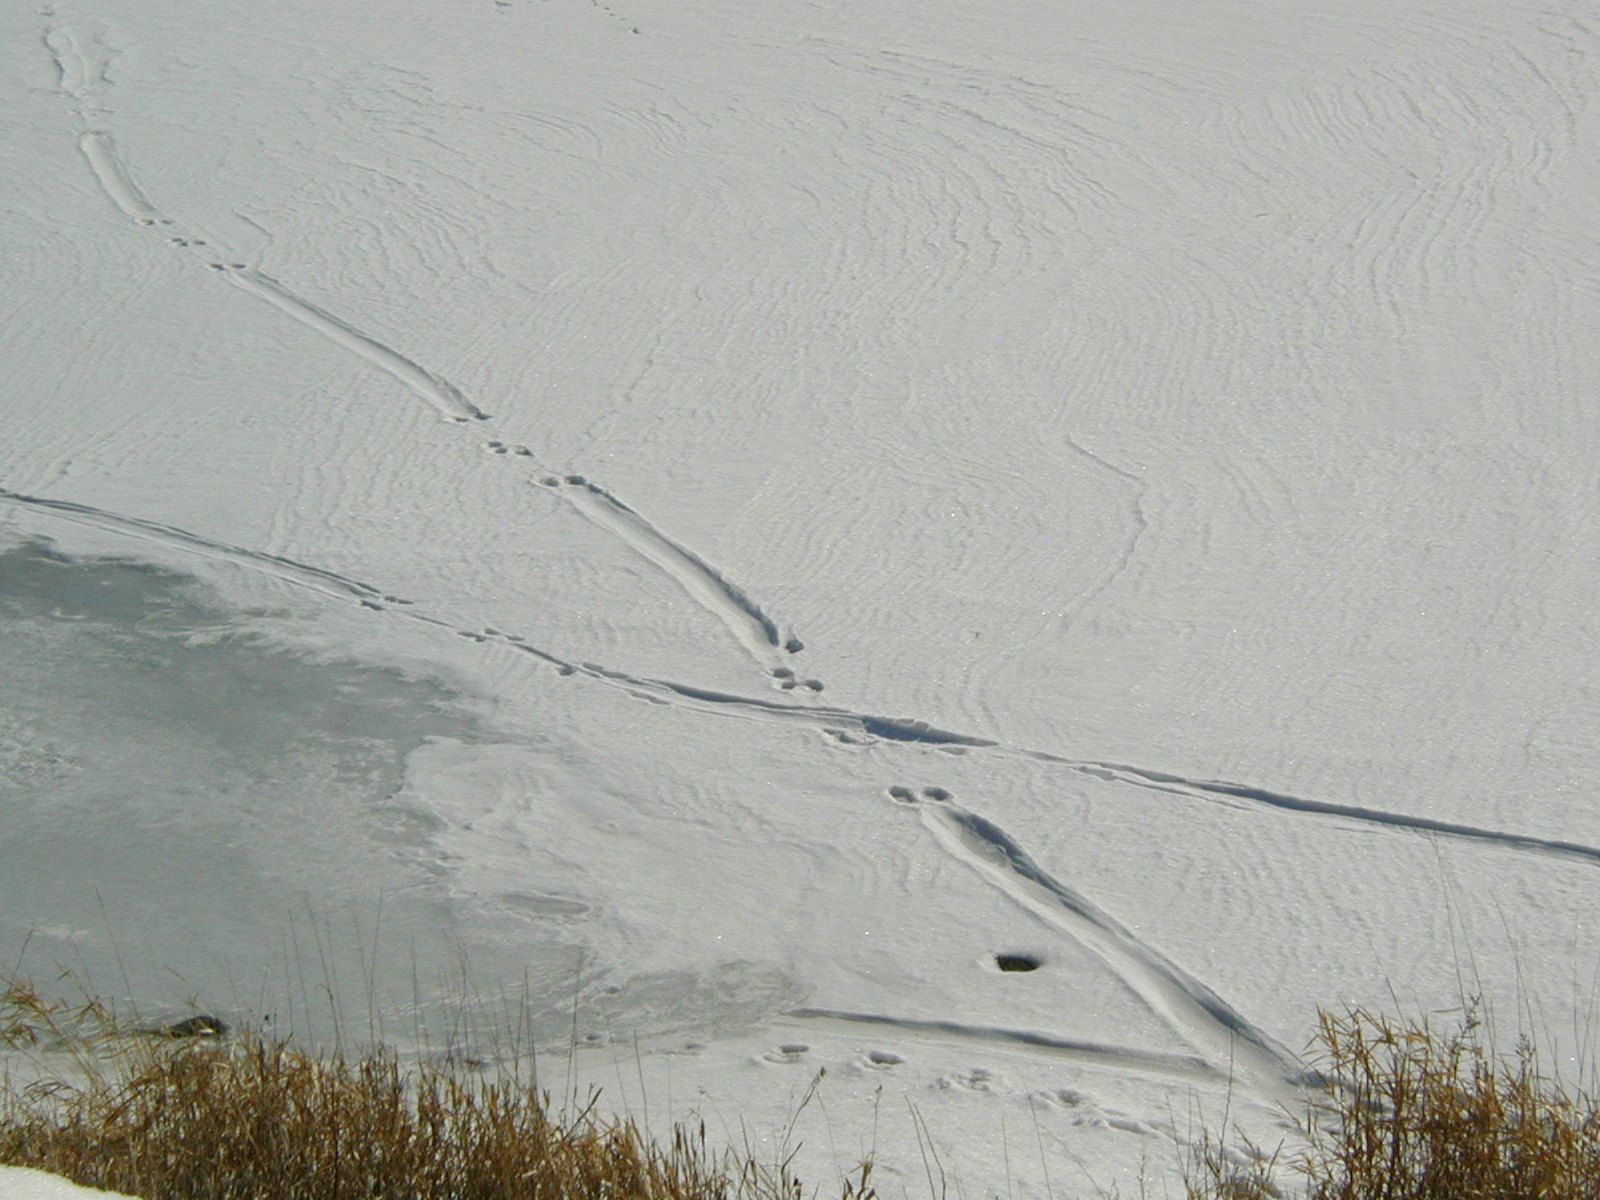
\includegraphics[width=\paperwidth]{ottertracks1.jpg}}
	\begin{frame}
		\titlepage
	\end{frame}
}

\begin{frame}{Outline}
		\tableofcontents[pausesections]
\end{frame}

\section{The data and questions}
\begin{frame}{Otters}
	\begin{columns}
		\column{5cm}
		\begin{itemize}[<+->]
			\item Otters endemic to all of Minnesota
			\item Indicator species for quality of aquatic habitat
			\item Populations crashed, now rebounding
			\item In SE Minnesota interest in resuming trapping
			\item Government needs tools to monitor changes in populations
		\end{itemize}
		\column{5cm}
		\resizebox{5cm}{!}{\includegraphics{cuteOtter1.pdf}}
	\end{columns}
\end{frame}

\begin{frame}{Map of area}
	\begin{picture}(310,190)(9,7.5)
		\put(20,-5){\resizebox{10cm}{!}{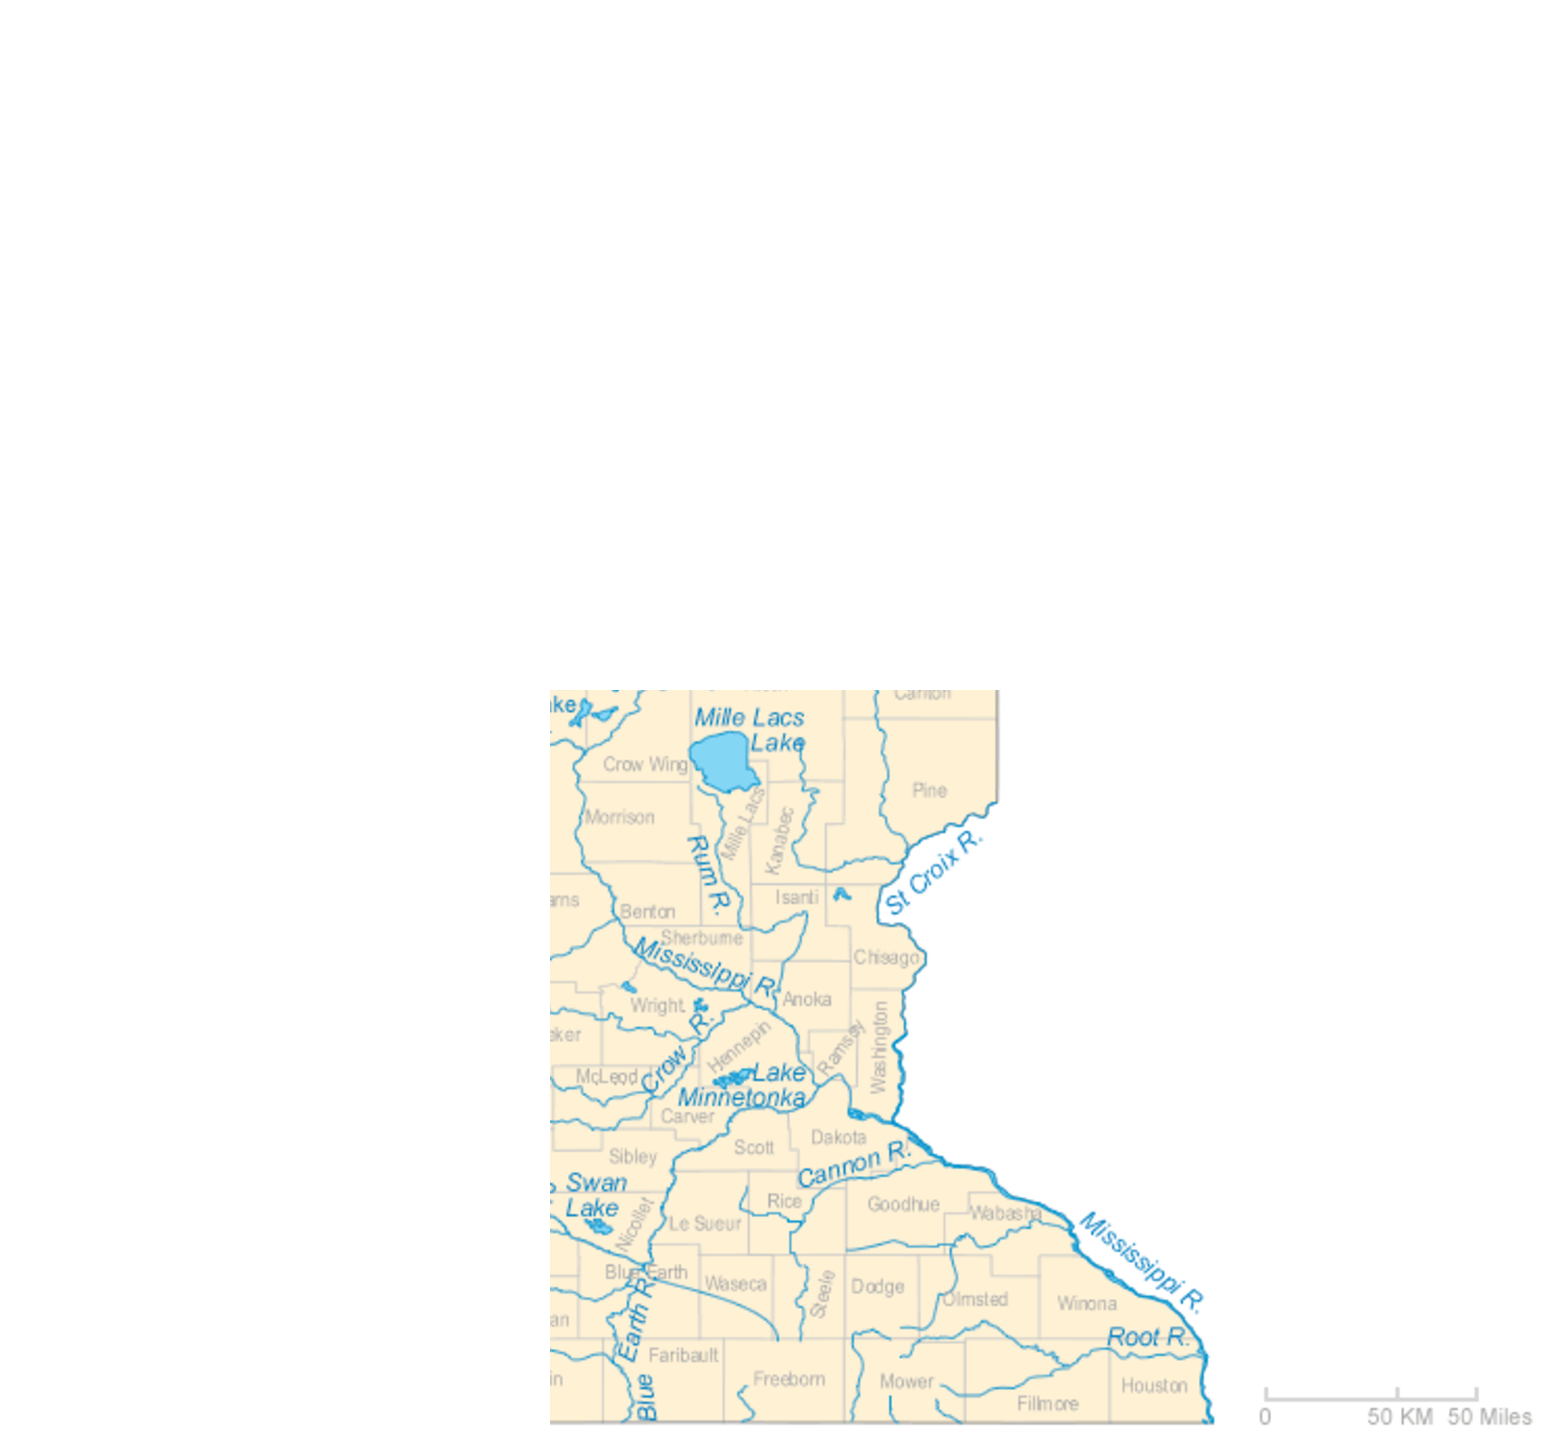
\includegraphics{map.pdf}}}
		%\graphpaper(0,0)(310,190)
        		\only<2>{\put(164,48){\circle{30}}}
   	\end{picture}
\end{frame}

\begin{frame}{Collecting data}
	\begin{columns}
		\column{5cm}
		\resizebox{5cm}{!}{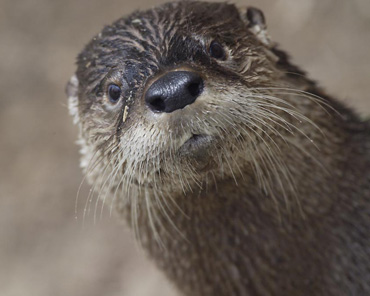
\includegraphics{cuteOtter2.jpg}}
		\column{5cm}
		\begin{itemize}[<+->]
			\item Researchers flew over rivers during winters of 2003, 2004
			\item Flew one, two, or three days after snow events
			\item Marked GPS coordinates of tracks
			\item Rivers divided into 402m, 804m, or 1608m plots
			\item Presence of track in each plot determined
			\item Also examined data set with every other plot excluded
			(Alternating Plots)
		\end{itemize}
	\end{columns}
\end{frame}

{
	\usebackgroundtemplate{
	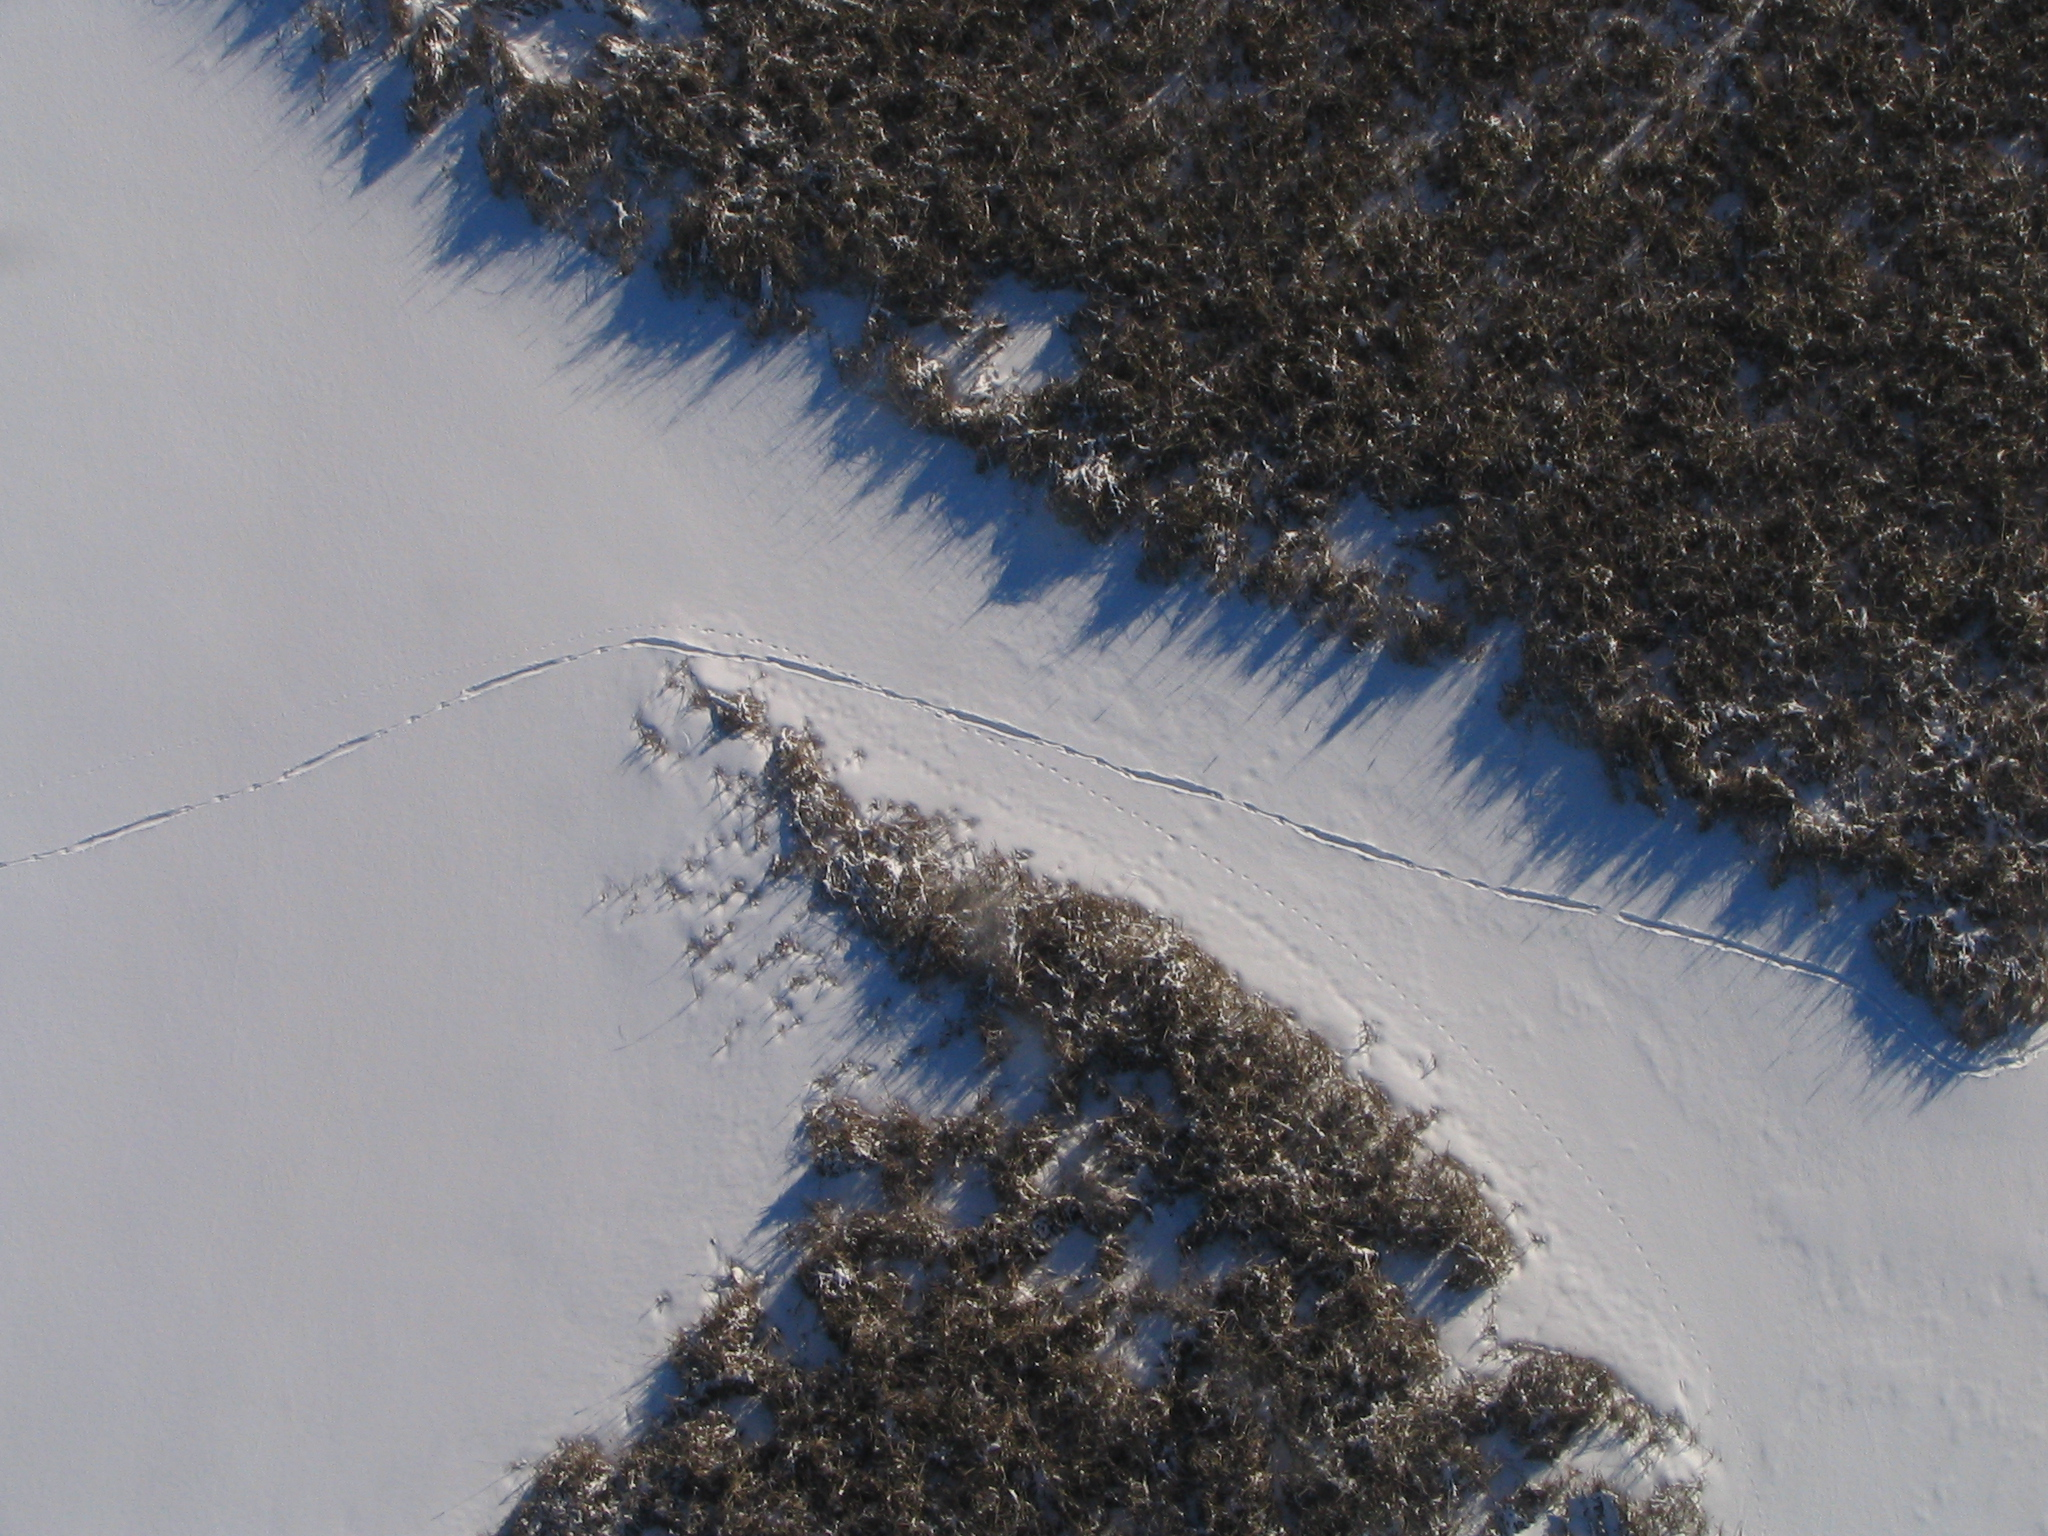
\includegraphics[width=\paperwidth]{SnowTracks12.jpg}}
	\begin{frame}{}
	\end{frame}
}

{
	\usebackgroundtemplate{
	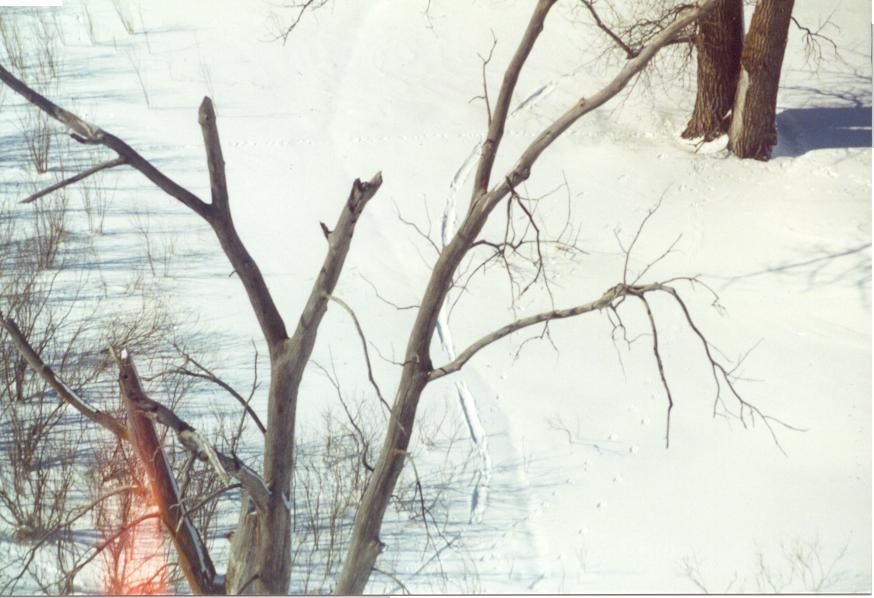
\includegraphics[width=\paperwidth]{SNOWTRACKS9.jpg}}
	\begin{frame}
	\end{frame}
}

{
\usebackgroundtemplate{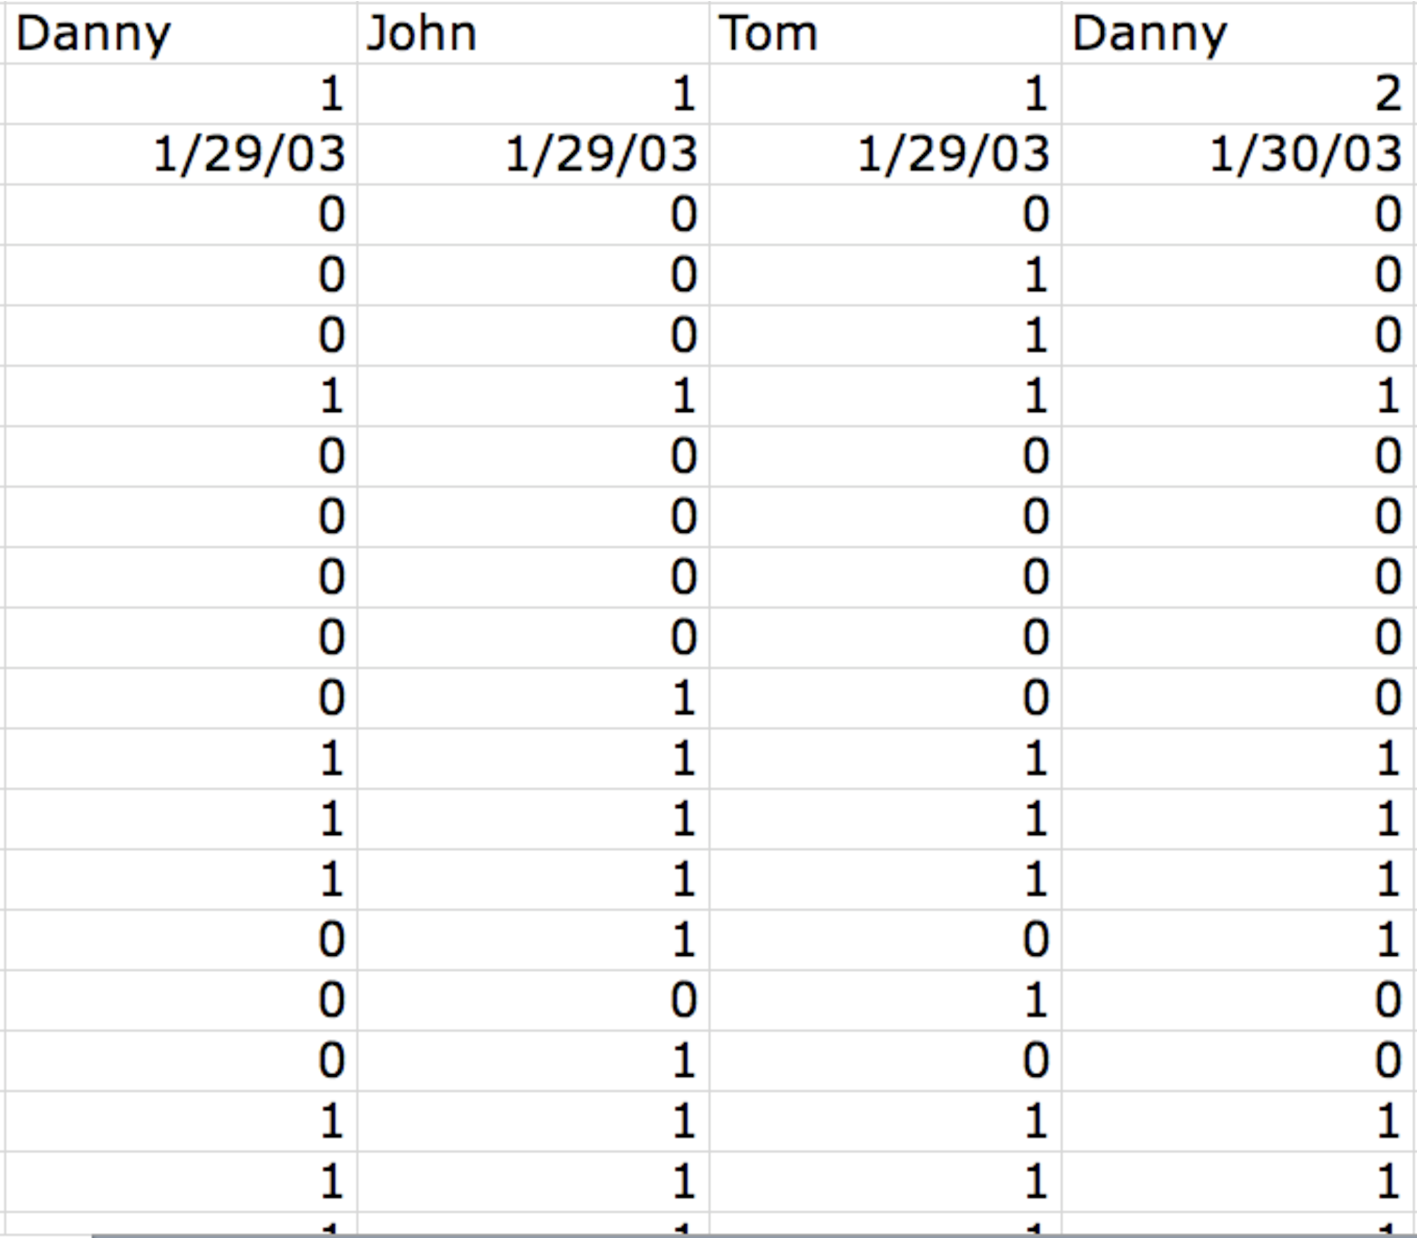
\includegraphics[width=\paperwidth]{data.pdf}}
\begin{frame}
    \begin{picture}(310,190)(9,7.5)
        \linethickness{1.5pt}
        \only<2->{\color<2>{red}\put(50,120){\framebox(290,15){}}}
        \only<3->{\color<3>{red}\put(150,-20){\framebox(15,80){}}}
        \only<4->{\color<4>{red}\put(150,-35){\framebox(103,30){}}}
    \end{picture}
\end{frame}
}

\section{Occupancy Theory}
\begin{frame}{Definitions of occupancy}
	\begin{itemize}
		\item The probability that a randomly selected site or sampling unit in
		an area of interest is occupied by a species
		\item The proportion of area, patches, or sampling units that is
		occupied
	\end{itemize}
	(MacKenzie, et al. 2006)
	\begin{center}
		\resizebox{5cm}{!}{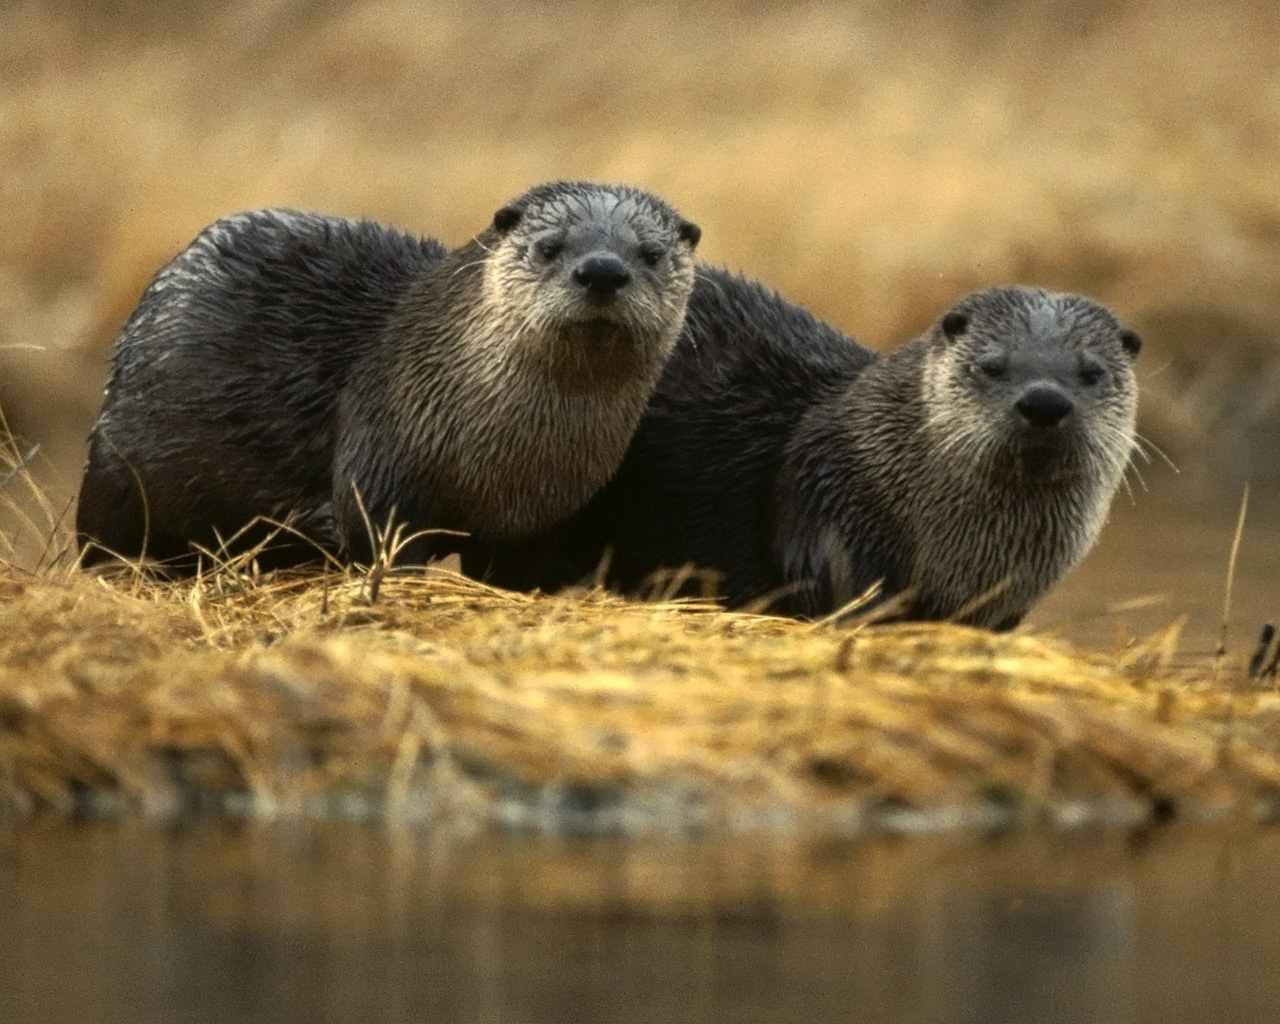
\includegraphics{cuteOtter3.jpg}}
	\end{center}
\end{frame}

\begin{frame}{Estimating occupancy}
	\begin{itemize}
		\item Ecologists often conduct surveys to find the occupancy rate
		\item Na\"ive occupancy: proportion of sites found to be occupied
		\item Not observing the species can mean two things:
		\begin{itemize}
			\item The species does not occupy the area
			\item The species went undetected during surveying
		\end{itemize}
		\item Need to be able to estimate probability of observing the species
		given its presence
	\end{itemize}
\end{frame}

\begin{frame}{Assumptions of occupancy models}
	\begin{columns}
		\column{5cm}
		\begin{itemize}
			\item No false positives
			\item Presence and detection probabilities are constant across sites
			and surveys (or can be modeled by covariates)
			\item Independence of detection between sites
			\item Survey is conducted on a closed population
		\end{itemize}
		\column{5cm}
		\resizebox{5cm}{!}{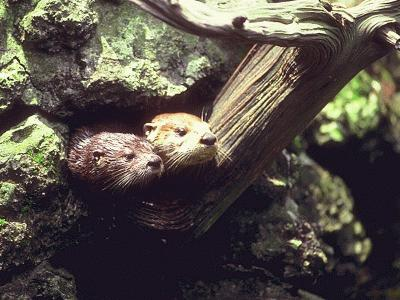
\includegraphics{cuteOtter4.jpg}}
	\end{columns}
\end{frame}

\begin{frame}{Types of occupancy models}
	\begin{itemize}
		\item Single species, single season
		\item Hierarchical models
	\end{itemize}
	\begin{center}
		\resizebox{7cm}{!}{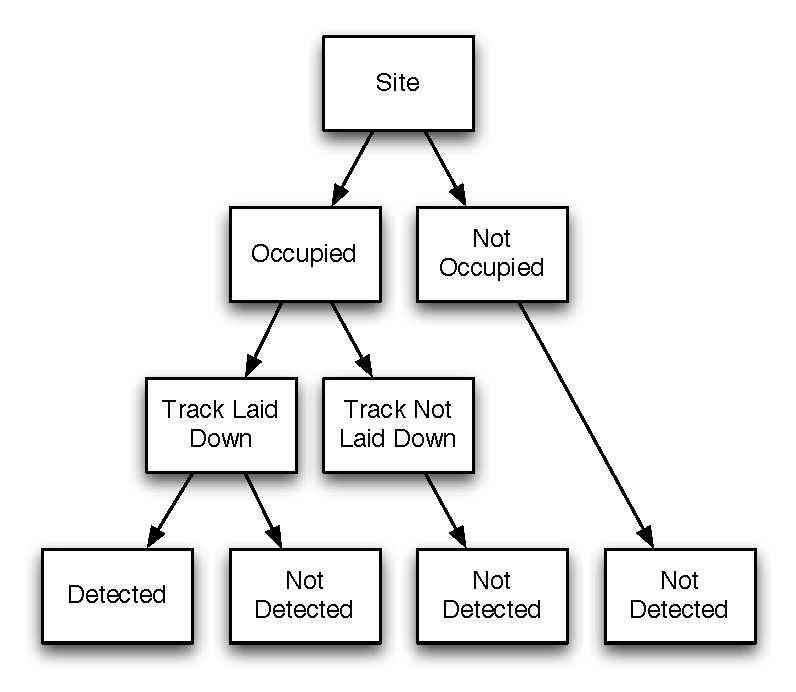
\includegraphics{../SimpleHierarchicalModel.pdf}}
	\end{center}
\end{frame}

\begin{frame}{Parameters}
	\begin{itemize}
		\item $\psi=$ The probability a site is occupied
		\item $\theta=$ The probability a track is laid down in a site on a
		given day, given that the site is occupied
		\item $p= $ The probability an observer sees a track given that a track
		has been made
	\end{itemize}
	\begin{center}
		\resizebox{7cm}{!}{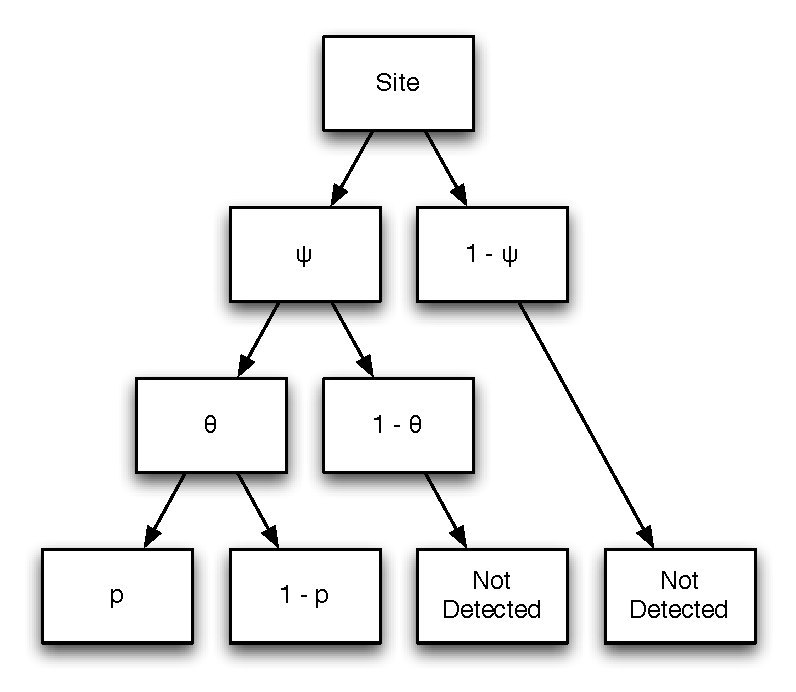
\includegraphics{../SimpleModelWithParams.pdf}}
	\end{center}
\end{frame}

\section{Exploring the data}
\begin{frame}{Effects of multiple observers}
	\begin{itemize}
		\item In 2003, three different observers
		\item Detection rates varied among the observers
	\end{itemize}
	\begin{center}
		\resizebox{5cm}{!}{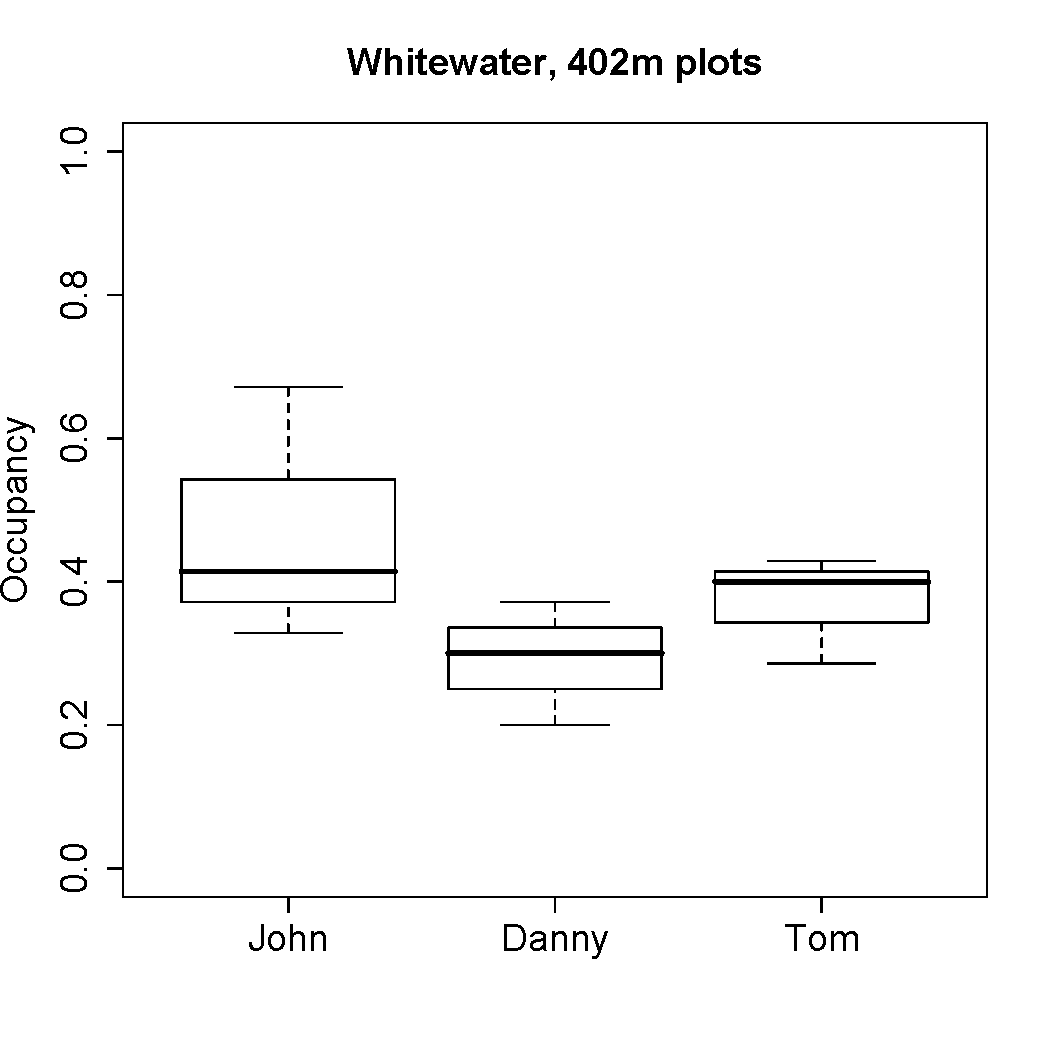
\includegraphics{wwObsPlot.pdf}}
	\end{center}
	\begin{itemize}
		\item Solution: use observer indicators as covariates for detection
		probability
	\end{itemize}
\end{frame}

\begin{frame}{Correlation between flights}
	\begin{center}
		\resizebox{7cm}{!}{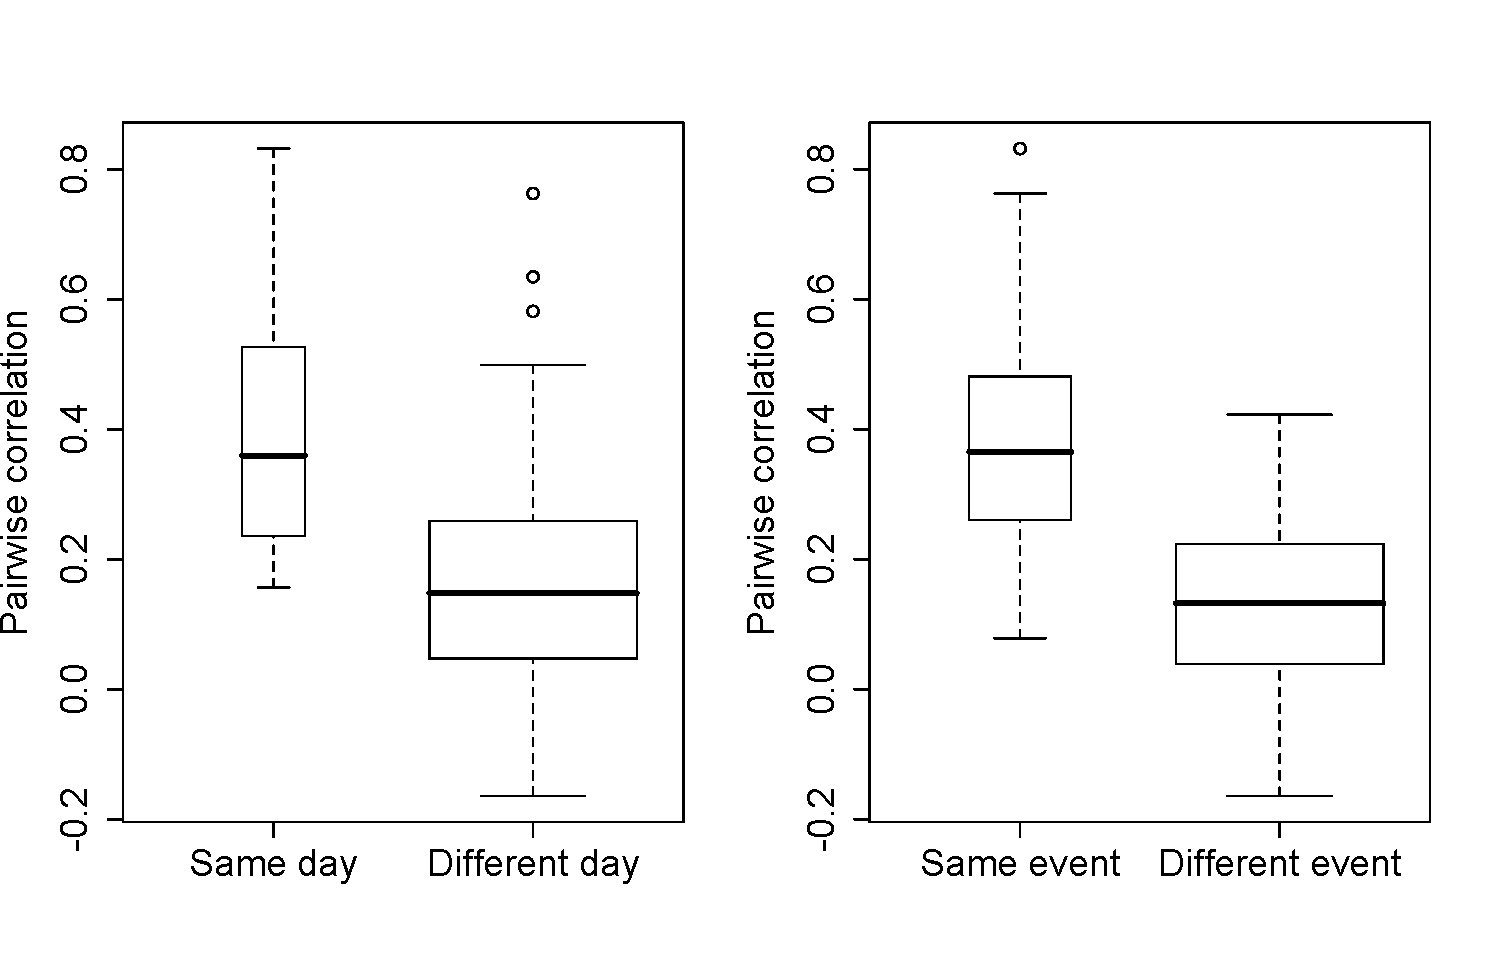
\includegraphics{dayEventGraphs.pdf}}
	\end{center}
	\begin{itemize}
		\item Also looked at correlation between flights
		\begin{itemize}
			\item Very low, overall
			\item Slightly higher during the same snow event or day
		\end{itemize}
		\item Solution: include false detection in model
	\end{itemize}
\end{frame}

\begin{frame}{Hierarchical model with false detection}
	\begin{center}
		\resizebox{10cm}{!}{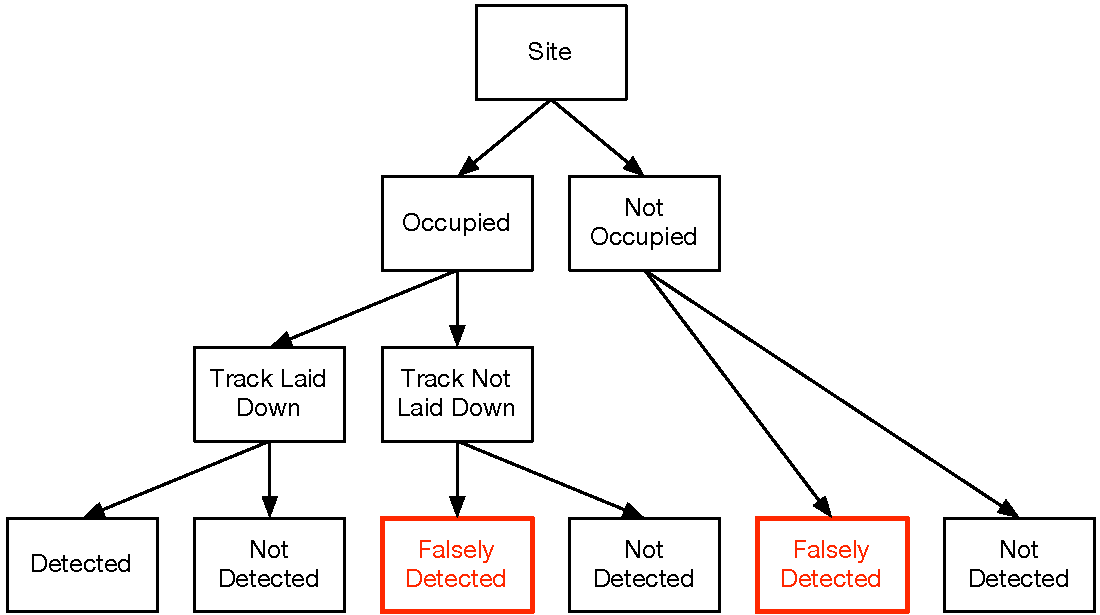
\includegraphics{../ModelWithE.pdf}}
	\end{center}
\end{frame}

\begin{frame}{Hierarchical model with false detection}
	\begin{center}
		\resizebox{10cm}{!}{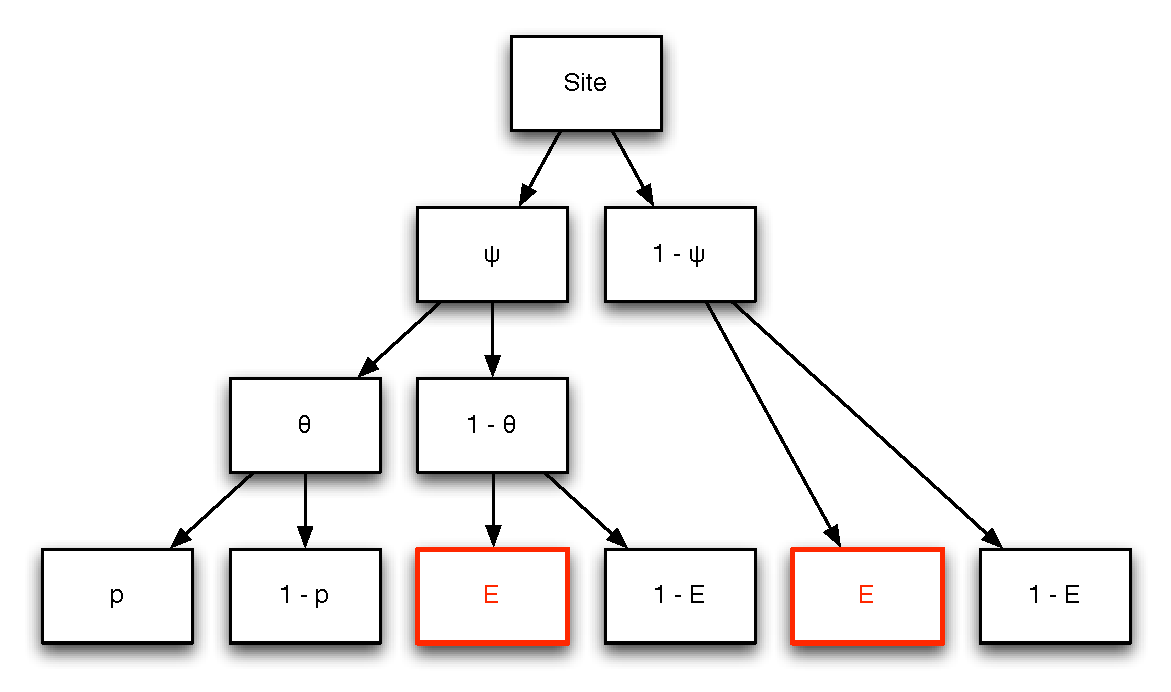
\includegraphics{../ModelWithEAndParams.pdf}}
	\end{center}
\end{frame}

\begin{frame}{Independence between plots}
	\begin{itemize}
		\item Assumption: independence between plots
		\item $S=(\text{\# of successive 0-1s})-(\text{\# of successive 1-1s})$
		\item Calculated $Z$-scores for each flight
			\begin{itemize}
				\item $Z=\frac{S-E[S]}{SD[S]}$
				\item $|Z_i|>2$ suggests assumption violated for flight $i$.
			\end{itemize}
	\end{itemize}
\end{frame}

\begin{frame}{Independence, continued}
	\begin{center}
		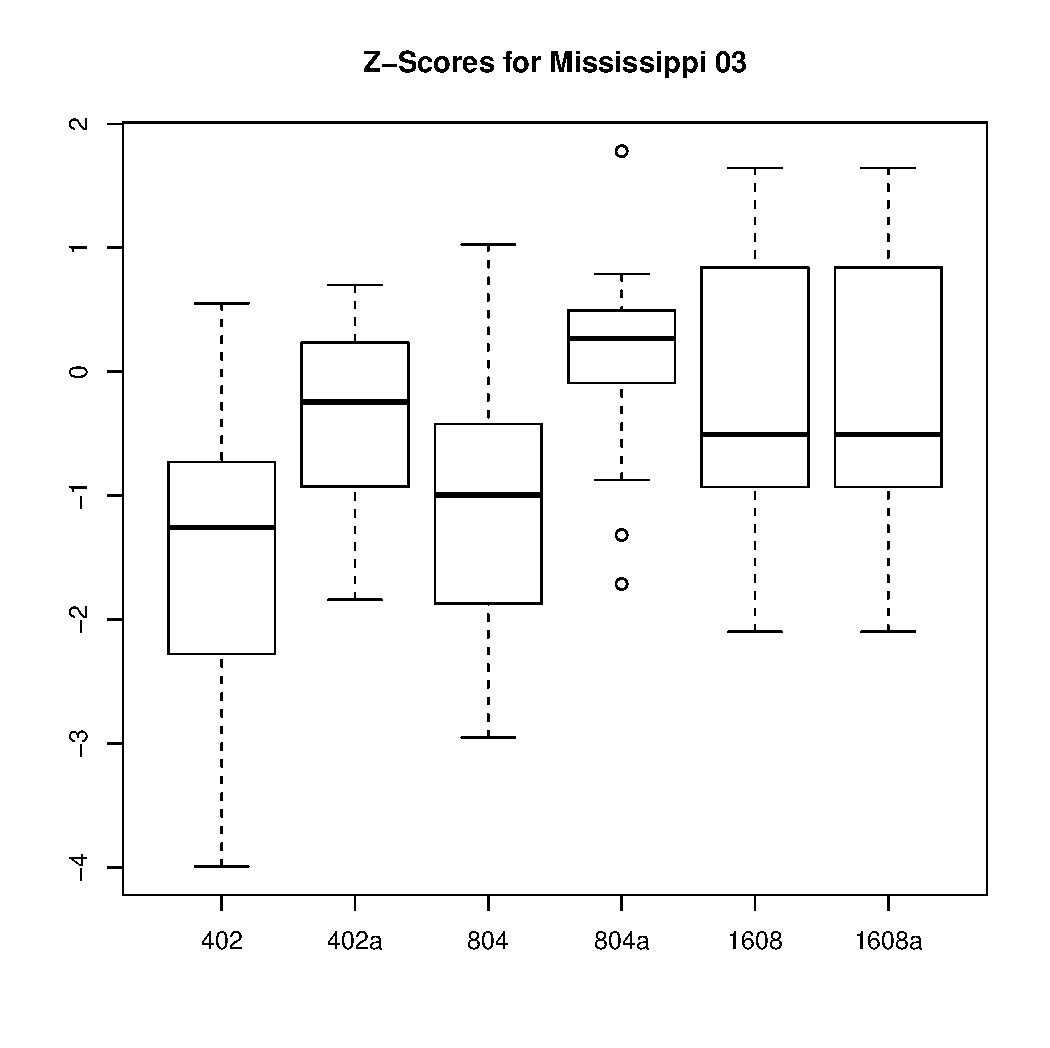
\includegraphics[scale=0.4]{independenceBoxplots.pdf}
	\end{center}
	\begin{itemize}
		\item Solution: keep issue in mind, include spatially dependent models
	\end{itemize}
\end{frame}

\section{Modeling the data}

\begin{frame}{Bayesian vs. likelihood occupancy models}
	\begin{itemize}
		\item Maximum likelihood assumes random sample from large population
		\begin{itemize}
			\item Entire section of river was sampled
		\end{itemize}
		\item Most occupancy models have two random processes -- occupancy and
		detection
		\begin{itemize}
			\item We added false detection and track-laying
			\item Extra parameters made likelihood model complicated
		\end{itemize}
		\item Spatial correlation is easier with a Bayesian model
	\end{itemize}
\end{frame}

\begin{frame}{Introduction to Bayesian statistics}
	\begin{itemize}
		\item Under Bayesian statistics, parameters are random variables
		\item According to Bayes' theorem
		\begin{itemize}
			\item $\text{posterior distribution} \propto \text{prior
			distribution}\times \text{likelihood}$
		\end{itemize}
		\item Goal: Estimate the posterior distribution
		\begin{itemize}
			\item Simulate a Markov Chain for many iterations
			\item Will approach true distribution of random variable
		\end{itemize}
	\end{itemize}
\end{frame}

\begin{frame}{Convergence}
	\begin{center}
		\resizebox{8.5cm}{!}{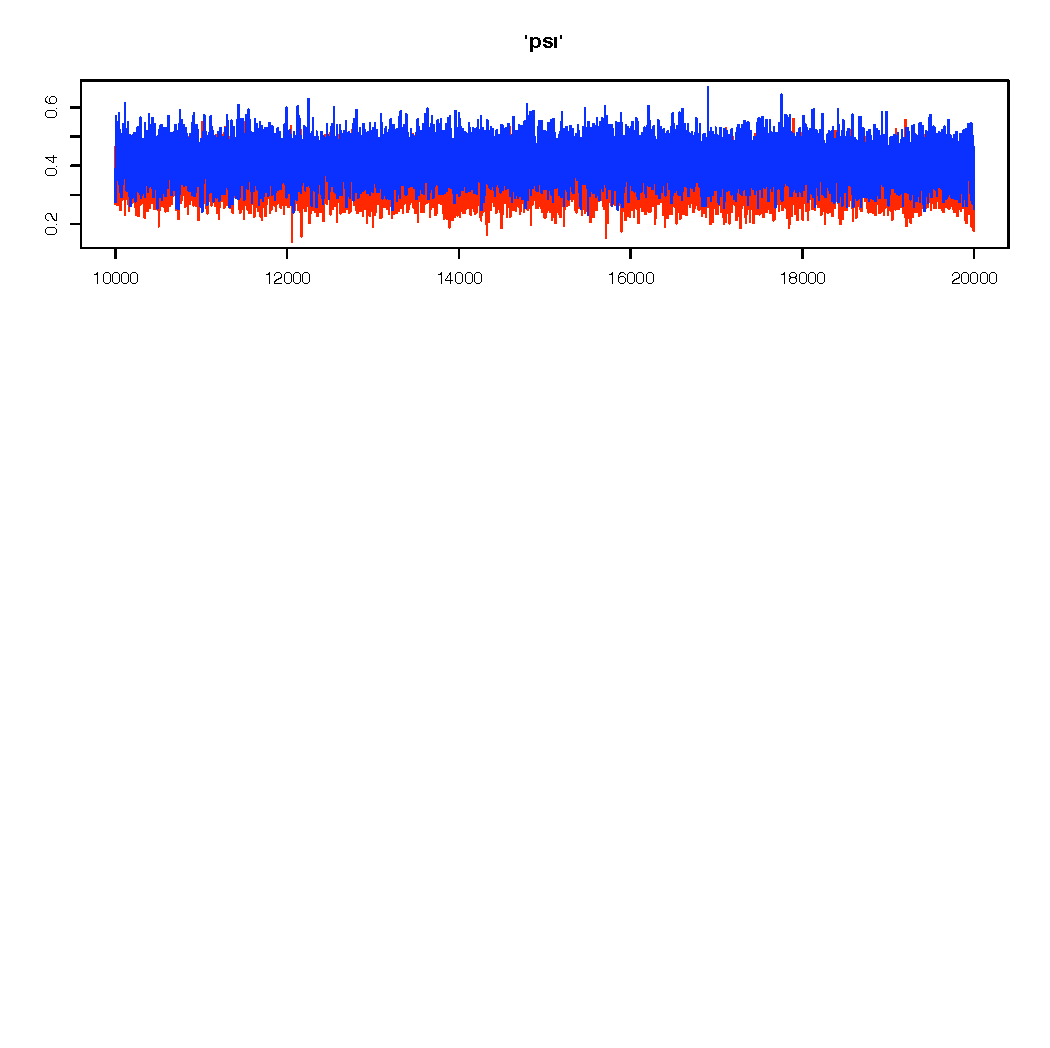
\includegraphics{historyConvergence.pdf}} \\
		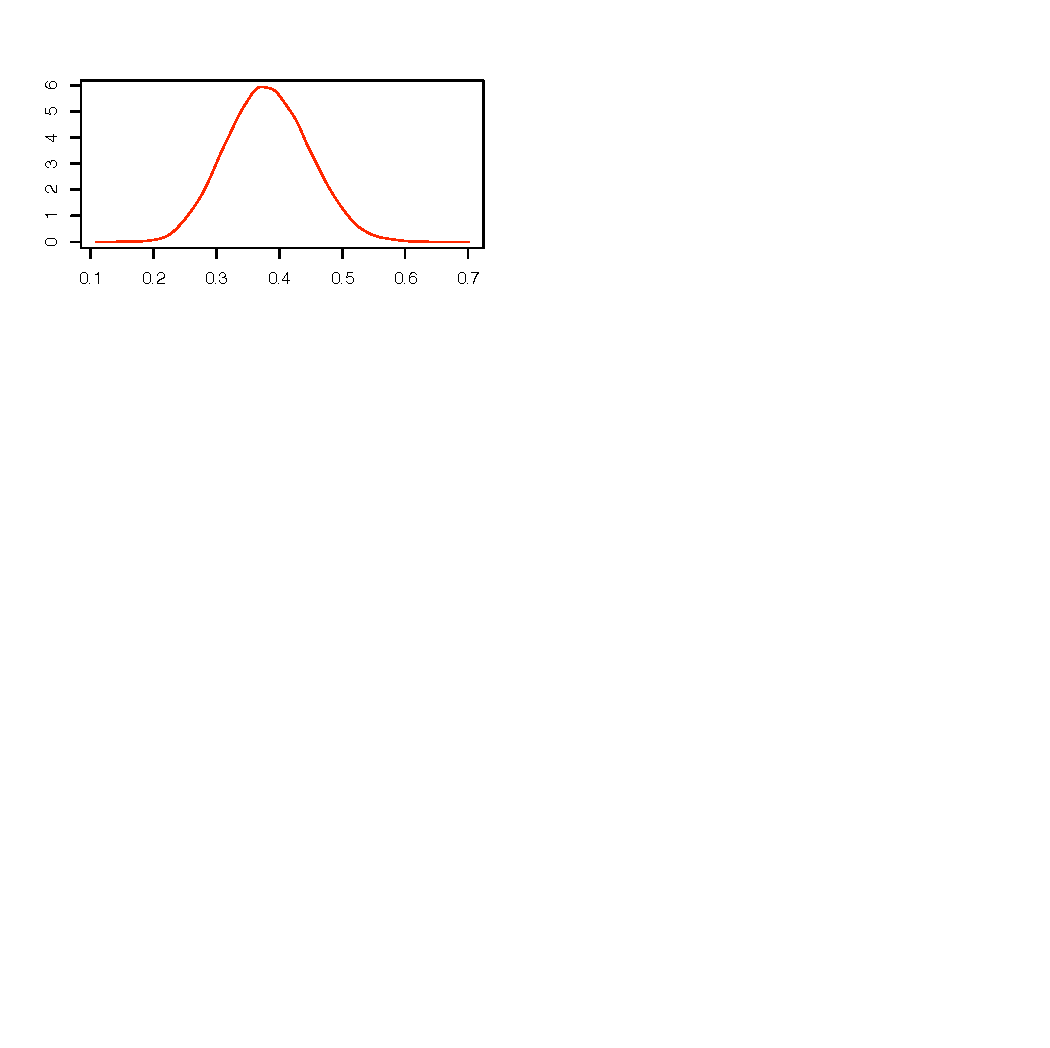
\includegraphics[scale=0.8]{distnConvergence.pdf} \\
	\end{center}
\end{frame}

\begin{frame}{Convergence}
	\begin{center}
		\resizebox{8.5cm}{!}{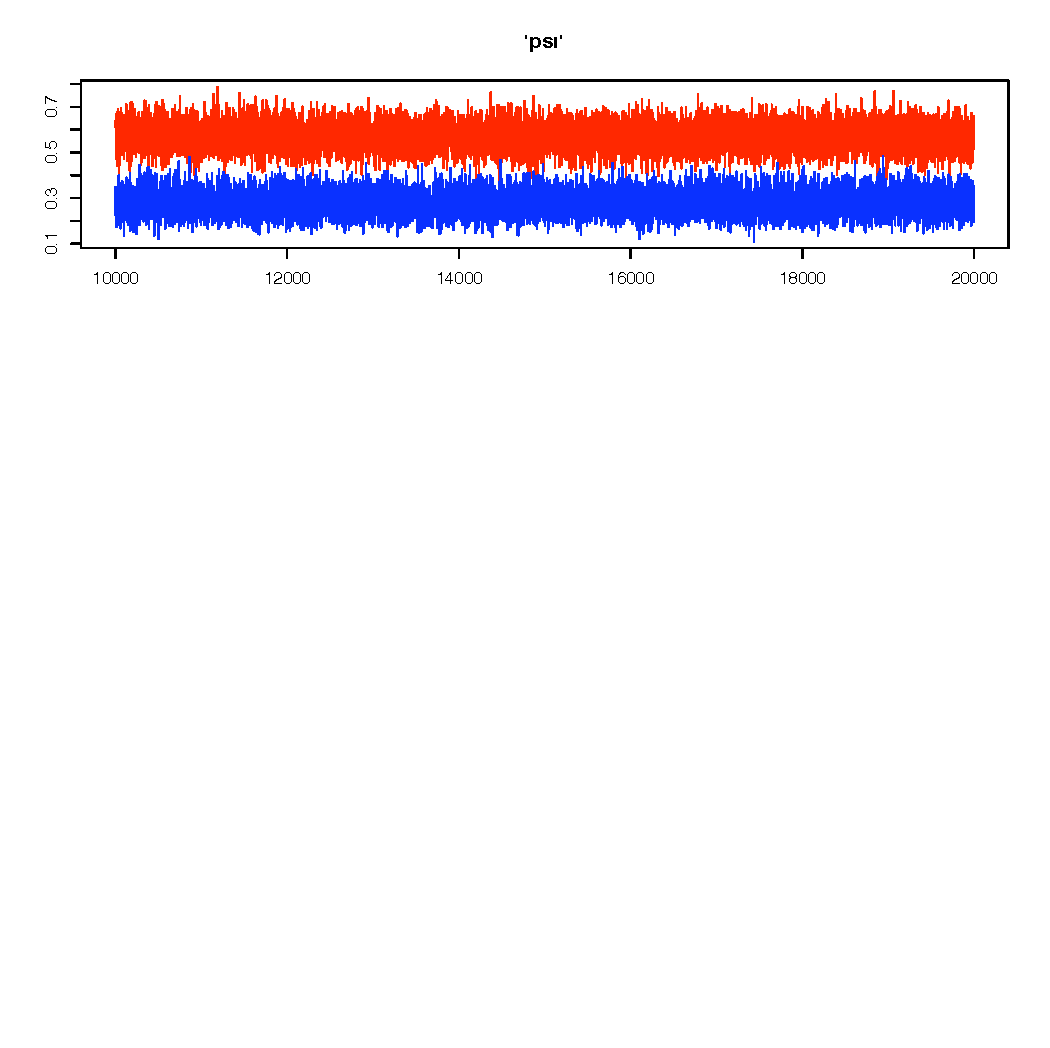
\includegraphics{historyNoConvergence.pdf}} \\
		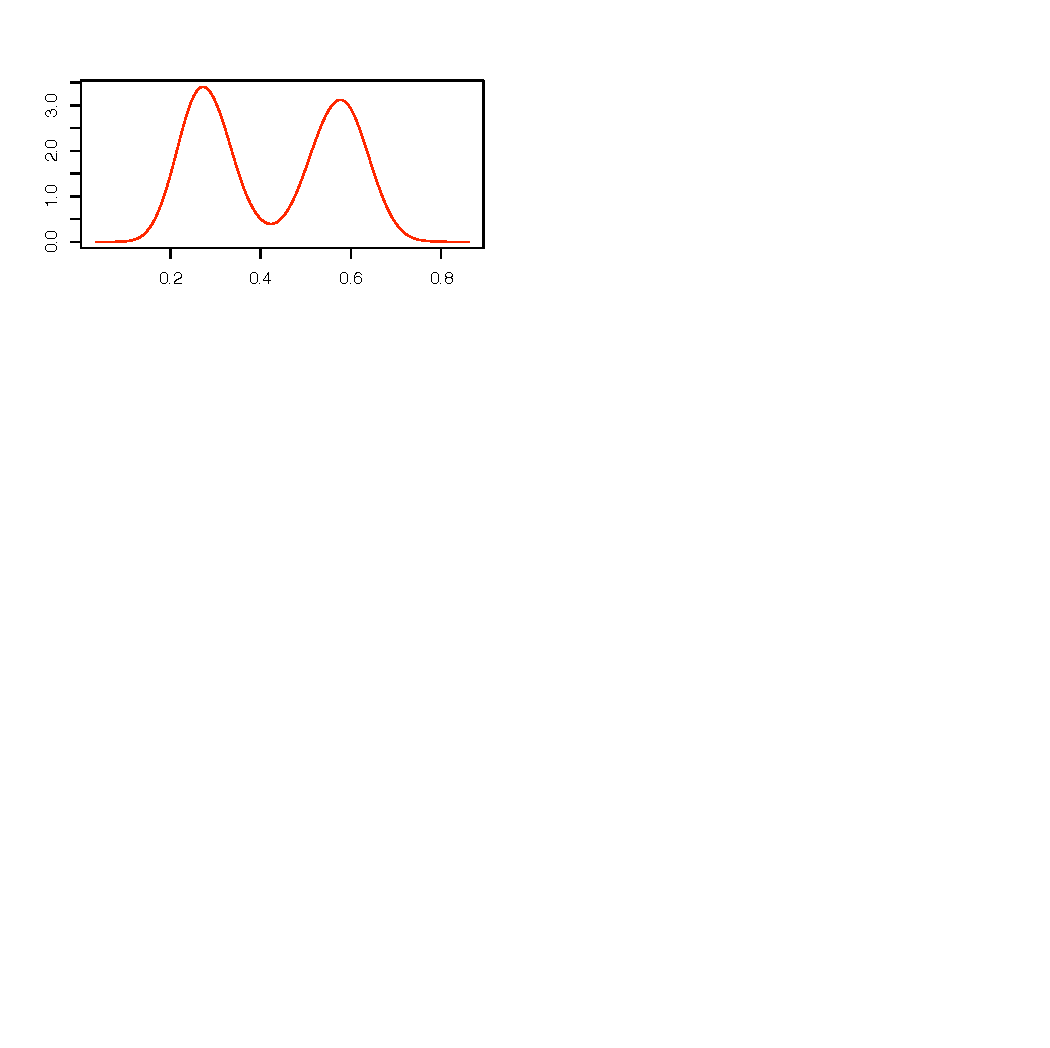
\includegraphics[scale=0.8]{distnNoConvergence.pdf} \\
	\end{center}
\end{frame}

\begin{frame}{Issue with false detection}
	\begin{columns}
		\column{5cm}
		\begin{itemize}
			\item $(p=x, E=y, \psi=z)$ equivalent in terms of likelihood to
			$(p=y,E=x,\psi=1-z)$.
			\item Leads to bimodal posterior distributions.
			\item Solution: restrict $p$ to interval $(0.6,1)$, $E$ to interval
			$(0,0.4)$.
		\end{itemize}
		\column{5cm}
		\resizebox{5cm}{!}{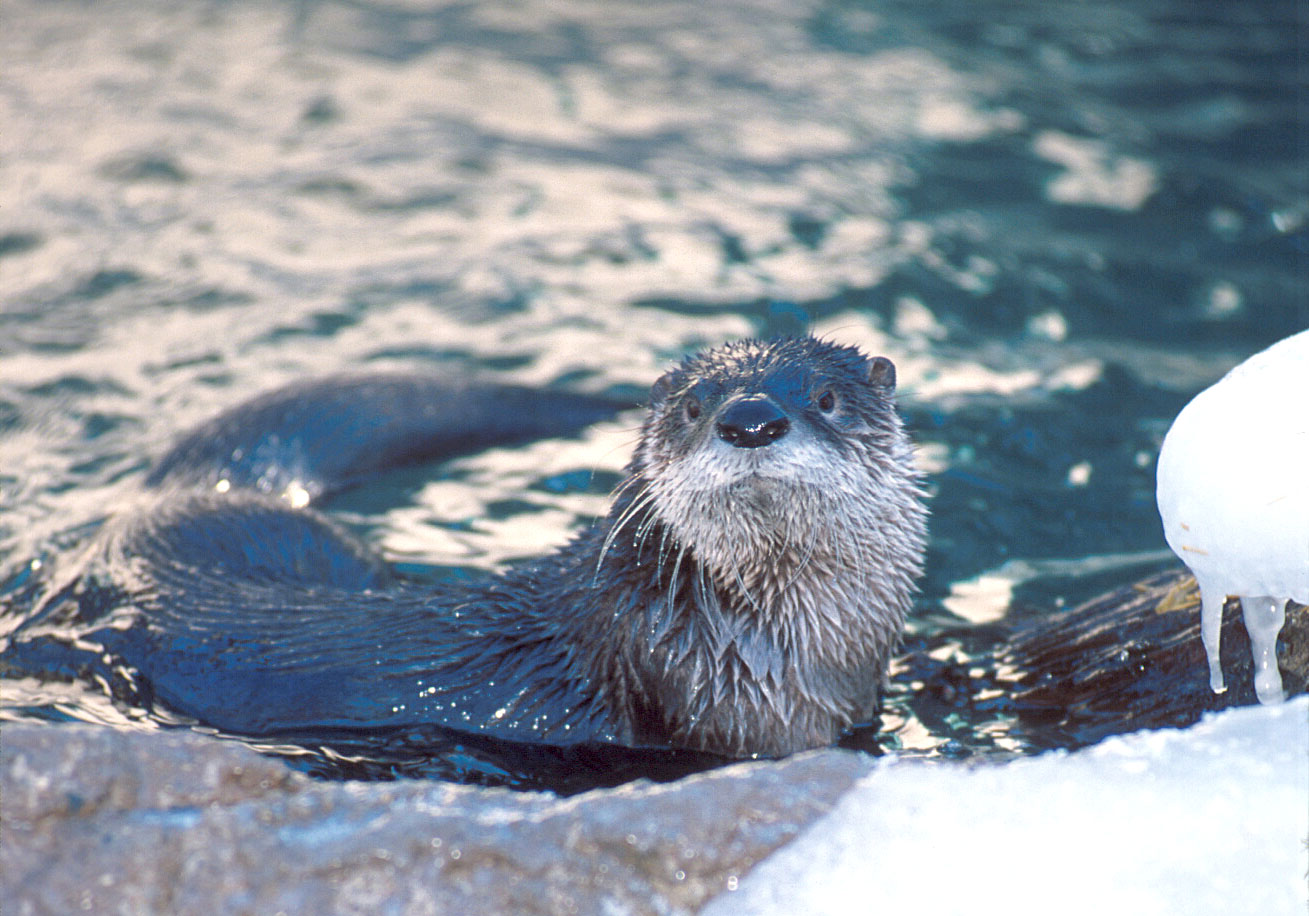
\includegraphics{cuteOtter6.jpg}}
	\end{columns}
\end{frame}

%This slide for DNR only
%\begin{frame}{Bayesian model specifics}
%	\begin{itemize}
%		\item $\psi,\theta \sim \text{Uniform}(0,1)$
%		\item $p[\text{obs}] \sim \text{Beta}(a,b)$
%		\begin{itemize}
%			\item $a, b \sim \text{Gamma}(1,0.1)$
%			\item E similar
%			\item $p$ and $E$ had restricted distributions
%		\end{itemize}
%		\item Burn-in period 10,000 iterations
%		\item Covariates: observer, days since snow
%	\end{itemize}
%\end{frame}

\begin{frame}{Testing the model -- data simulations}
	\begin{itemize}
		\item Simulated data with known $\psi$, $\theta$, $p$, $E$.
		\item To simplify, every observer flew every day, flights ran all
		three days after a snow event
		\item Ran data on our model
		\item When regularity restriction lifted, similar results
	\end{itemize}
\end{frame}

\begin{frame}{Testing the model, continued}
	\begin{center}
	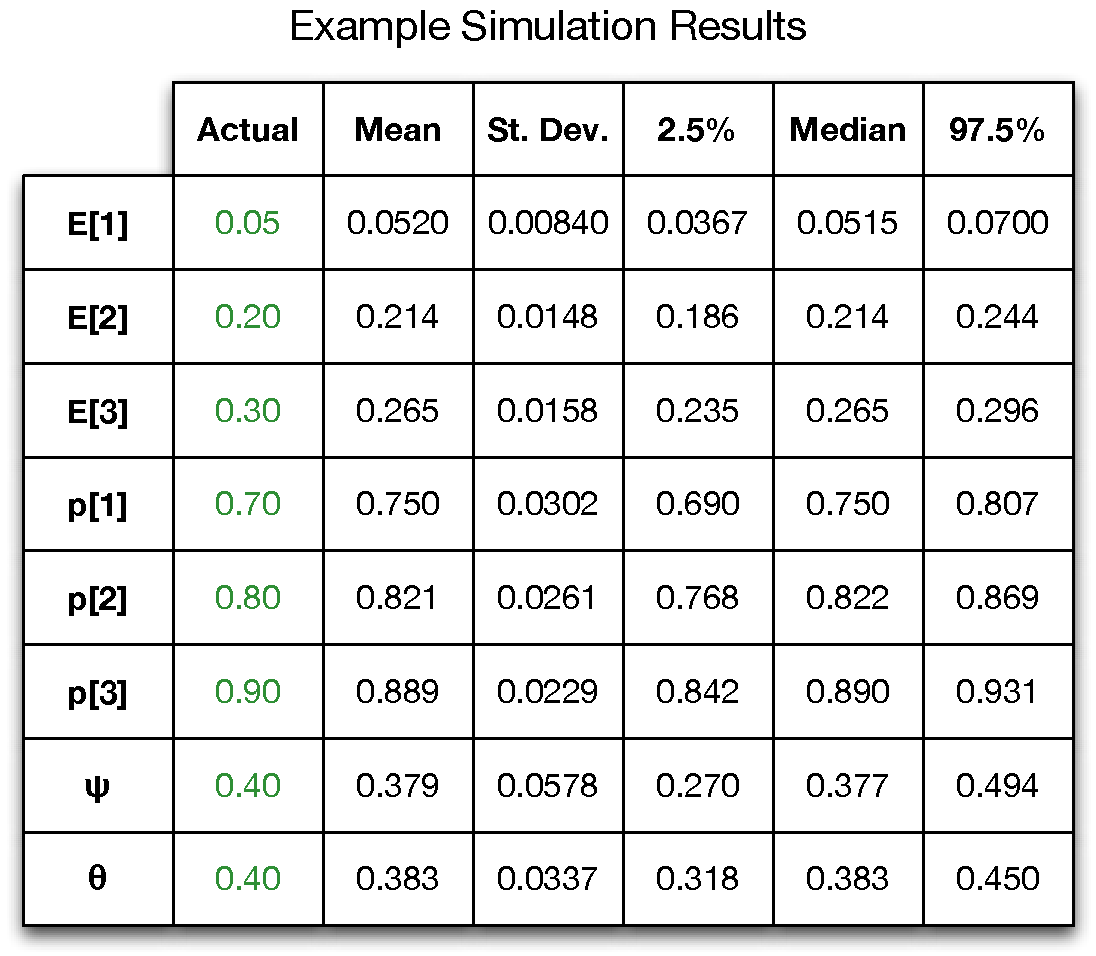
\includegraphics[scale=0.5]{../SimulatedData.pdf}
	\end{center}
\end{frame}

\begin{frame}{Results from simulated data}
	\begin{itemize}
		\item Lower values for $\psi$ and $\theta$ had better convergence and
		estimates
		\item 95\% confidence interval about 0.2 units wide
		\item Estimates usually within 0.1 of actual value
		\item Overall, model estimates parameters well
	\end{itemize}
\end{frame}

\begin{frame}{Modeling spatial correlation}
	\begin{itemize}
		\item Conditional autoregressive (CAR) models
		\item Allows extreme values to influence estimates of neighboring sites
		\item Placed CAR prior on $\theta$, track-laying probability
		\item With CAR model, each site has a unique estimate of $\theta$
	\end{itemize}
\end{frame}

%DNR only slide
%\begin{frame}{CAR model specifics}
%	\begin{itemize}
%		\item $\tau^2 =$ conditional variance
%		\item $(\tau^2)^{-1} \sim \text{Gamma}(0.5,0.0005)$
%		\item $\text{logit}(\theta_s)=\alpha_0+\alpha_{1_s}$
%		\item $\alpha_0 \sim$ Improper uniform
%		\item $\alpha_1 \sim$ Gaussian CAR
%	\end{itemize}
%\end{frame}

\begin{frame}{Testing the CAR model}
	\begin{itemize}
		\item Simulated data with correlation in $\theta$
		\begin{itemize}
			\item $P(\text{track in site }i|\text{no track in site }i-1)=\theta$
			\item $P(\text{track in site }i|\text{track in site }i-1)=\theta+
			\alpha$
		\end{itemize}
		\item CAR model did not converge
		\item Simulated data less dependent than actual data (from $S$)
		\item Added similar correlation in $\psi$
		\begin{itemize}
			\item CAR model converged more often
			\item Dependence more similar to that of actual data
		\end{itemize}
		\item When CAR model converged, estimates from CAR and standard models
		similar for the same data
	\end{itemize}
\end{frame}

\section{Discussion}
\begin{frame}{Obtaining convergence on the data}
	\begin{itemize}
		\item All of 2003 data converged with standard model
		\item None of 2004 data converged with standard model
		\begin{itemize}
			\item Removed false detection. 2004 data with 402m plot size
			converged, but estimates not dependable
		\end{itemize}
		\item CAR model never converged with $E$. Without $E$, poor
		estimates for $\psi$
	\end{itemize}
\end{frame}

\begin{frame}{}
    % Mississippi River!
	\small{
    \begin{table}
    \begin{center}
    \begin{tabular}{|l|l|l|l|}
        \hline
        \multicolumn{4}{|l|}{\textbf{Mississippi River, 2003}} \\
        \hline
            & 402m & 804m & 1608m \\
        \hline
        \multirow{2}{*}{E[Danny]}
            & 0.01954 & 0.04808 & 0.06885 \\
            & (0.006515, 0.03663) & (0.01874, 0.08187) & (0.01778, 0.1383) \\
        \hline
        \multirow{2}{*}{E[John]}
            & 0.05216 & 0.07771 & 0.13650 \\
            & (0.027710, 0.07745) & (0.03881, 0.12100) & (0.03449, 0.2330) \\
        \hline
        \multirow{2}{*}{E[Tom]}
            & 0.02668 & 0.06140 & 0.10230 \\
            & (0.011990, 0.04622) & (0.02789, 0.10390) & (0.04287, 0.1796) \\
        \hline
        \multirow{2}{*}{p[Danny]}
            & 0.65240 & 0.67340 & 0.74960 \\
            & (0.548300, 0.75990) & (0.56760, 0.78290) & (0.60510, 0.8910) \\
        \hline
        \multirow{2}{*}{p[John]}
            & 0.67770 & 0.77580 & 0.82540 \\
            & (0.583500, 0.77280) & (0.66060, 0.88690) & (0.71390, 0.9326) \\
        \hline
        \multirow{2}{*}{p[Tom]}
            & 0.53670 & 0.54220 & 0.65330 \\
            & (0.501200, 0.61300) & (0.50160, 0.62850) & (0.51530, 0.8104) \\
        \hline
        \multirow{2}{*}{\(\psi\)}
            & 0.59380 & 0.69370 & 0.75820 \\
            & (0.439000, 0.75990) & (0.51800, 0.87380) & (0.54110, 0.9300) \\
        \hline
        \multirow{2}{*}{\(\theta\)}
            & 0.15280 & 0.20730 & 0.27690 \\
            & (0.111900, 0.19780) & (0.14580, 0.27390) & (0.19030, 0.3716) \\
        \hline
    \end{tabular}
    \end{center}
	\end{table} 
	}
\end{frame}

% Add slide with example of estimates for our actual data, one river/year?

\begin{frame}{Summary and interpretation of estimates}
	\begin{itemize}
		\item Estimates for all parameters increase with plot size
		\item Possible hypotheses:
		\begin{itemize}
			\item \(\psi\) and \(\theta\)
			\item \(p\) and \(E\)
		\end{itemize}
		\item Used data from all plots, not alternating plots
		\begin{itemize}
			\item More data more useful than more independence
		\end{itemize}
	\end{itemize}
	\begin{center}
		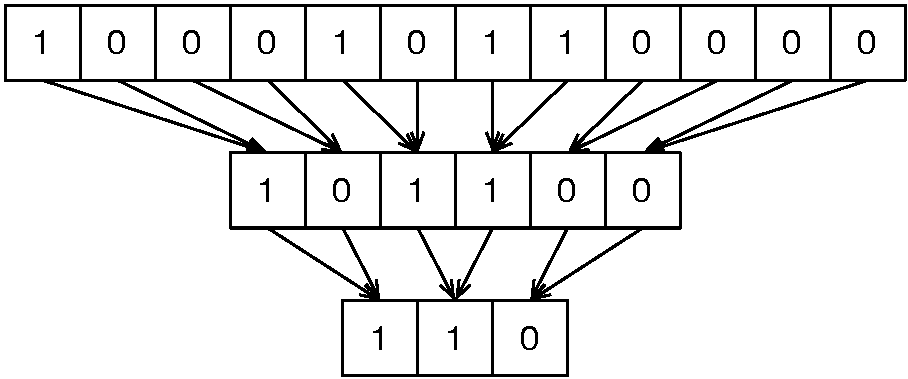
\includegraphics[scale=0.5]{Aggregation.pdf}
	\end{center}
\end{frame}

\begin{frame}{Recommended sampling practices}
	\begin{itemize}
		\item Investigated effects of changing the sampling variables
		\item In order of decreasing importance, maximize:
		\begin{enumerate}
			\item Number of consecutive days after snow event sampled
			\item Number of snow events
			\item Number of observers
		\end{enumerate}
		\item We suggest: 1 observer, 3 snow events, 3 days since snow
		\item All conclusions come from regular data
	\end{itemize}
\end{frame}

\begin{frame}{Acknowledgments}
	\begin{itemize}
		\item Bob Dobrow, adviser
		\item John Fieberg, MN DNR
		\item John Erb, MN DNR
	\end{itemize}
	\begin{center}
		\resizebox{7cm}{!}{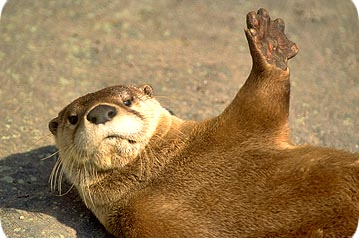
\includegraphics{cuteOtter10.jpg}}
	\end{center}
\end{frame}

\begin{frame}{Questions?}
	\begin{center}
	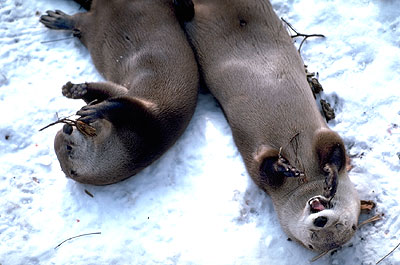
\includegraphics[scale=0.7]{cuteOtter7.jpg}
	\end{center}
\end{frame}

\end{document}